\documentclass[11pt,a4paper]{article}
\usepackage[utf8]{inputenc}
\usepackage{amsmath, amssymb, amsthm}
\usepackage{geometry}
\usepackage{fancyhdr}
\usepackage{hyperref}
\usepackage{graphicx}
\usepackage{enumitem}
\usepackage{color}
\usepackage{titlesec}
\usepackage{enumerate}

% Set the page geometry
\geometry{a4paper, margin=1in}

% Customize the header and footer
\pagestyle{fancy}
\fancyhf{}
%\fancyhead[L]{\textbf{Lecture Title}}
%\fancyhead[R]{\textbf{Date}}
\fancyfoot[C]{\thepage}

% Title format
\titleformat{\section}
  {\normalfont\Large\bfseries}{\thesection}{1em}{}
\titleformat{\subsection}
  {\normalfont\large\bfseries}{\thesubsection}{1em}{}

% Define theorem styles
\newtheorem{theorem}{Theorem}[section]
\newtheorem{definition}[theorem]{Definition}
\newtheorem{lemma}[theorem]{Lemma}
\newtheorem{corollary}[theorem]{Corollary}
\newtheorem{proposition}[theorem]{Proposition}
\newtheorem{example}[theorem]{Example}

% Custom commands
\newcommand{\R}{\mathbb{R}}
\newcommand{\N}{\mathbb{N}}
\newcommand{\Z}{\mathbb{Z}}
\newcommand{\Q}{\mathbb{Q}}
\newcommand{\C}{\mathbb{C}}
\newcommand{\E}{\mathbb{E}}
\newcommand{\Var}{\text{Var}}
\newcommand{\Tr}{\text{Tr}}

\begin{document}

\title{Lecture Notes on Exact solutions}
\author{Simran Singh}
\date{21 May 2024}
\maketitle

\tableofcontents
\newpage

\section{Introduction}

For the first part of the lecture we will use the \emph{energy-entropy} argument to understand why the lower critical dimension of the Ising model is $d_c = 1$. This means that the model does not undergo a phase transition at any \emph{finite} temperature for the 1D Ising chain. For this we will study the system with nearest neighbour ferromagnetic interactions. We will further use the fact that in order to discuss the presence of a phase transition we must study systems in the thermodynamic limit, \emph{i.e.,} $N \to \infty$. We will also consider the system with no external magnetic field, since a phase transition only exists in this case. \\

For the second part of the lecture we will see some exact solutions of the $1$D Ising chain in the presence an absence of an external magnetic field. We will again discuss the non-existence of phase transitions using the Transfer matrix formalism.

\section{Landau \& Peierl's argument}
Peierl (1936) and Landau (1969) gave heuristic arguments for the non-existence of phase transitions in some 1D systems. The argument will be explained here starting from the absence of \emph{long range order} at any finite T, in the 1D Ising chain. For this consider we will consider the Free energy of the system given by:

\begin{equation}
     F = E - T S \,,
\end{equation}
 where $E$ is the internal energy of the system given by $-\sum_{i} S_i S_{i+1}$ and $S$ is the entropy given by $k_B \log{n}$. The significance of $n$ is related to counting configurations of spin that give the same energy, as explained below.  

When we consider the system at $T=0$, the free energy is minimized by minimizing $E$, and hence all spins align either all up or all down. However, at any finite $T$, the contribution of the entropy to the free energy is non-zero. In this situation, the system minimizes free energy by maximising the entropy $S$. We also know that for magnetic systems showing a phase transition from paramagnetic to ferromagnetic phase, there is a formation of domains when $T < T_c$. These domains characterize long range order. Hence, in order to show that the 1D Ising chain does not have a phase transition we will show why there can be no formation of \emph{stable} domains for any $T > 0$, in the thermodynamic limit. We will start by assuming that we have a domain present as in Fig. \ref{fig:1DPeierl} for $T > 0$ and show that such a state is \emph{unstable} under thermal fluctuations.

\begin{figure}[ht]
    \centering
    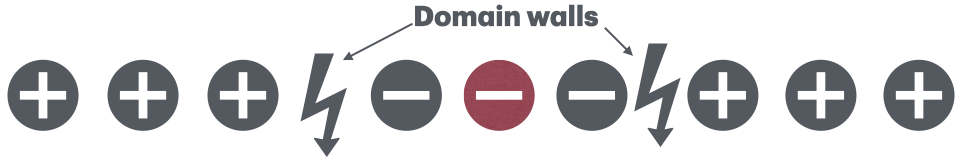
\includegraphics[scale=0.25]{PeierlsArg.png}
    \caption{1D Ising chain with domains}
    \label{fig:1DPeierl}
\end{figure}

To see this, consider the energy of the system at $T=0$, which is given by $F = E = -N J $, for $N$ spins in which (say) all spins point up (positive). The change in the free energy of this system when we introduce a domain of down spins centered at the coloured spin, as in Fig. \ref{fig:1DPeierl} is given by 

\begin{align*}
      \Delta F &= \Delta E - T S \nonumber \\
    \Delta E &= 4 J \,
\end{align*}
The entropy can be computed by asking in how many ways we can move the domain of down (negative) spins while including the coloured spin, to maintain the same energy. This is given by the length of the domain, which in Fig. \ref{fig:1DPeierl} is $3$. This gives us the change in free energy,

\begin{equation}
    \Delta F = 4 J - T k_B \log{n}
\end{equation}

This implies that for any $T > 0$, we can find a domain of length $n$, that lowers the free energy of the system. In the thermodynamic limit $N \to \infty$, this means $\Delta F \to -\infty$ as $N \to \infty$. The system can lower its free energy by creating multiple domain walls, hence states with long range order are unstable and the system is driven toward disorder by introducing thermal fluctuations. \\

\noindent \textbf{Note:} Two ingredients made the above argument possible, the short-range interaction and the fact that in $1$D, an increase in energy does not depend on the length of the domain introduced but only depends on the number of domains, whereas the entropy grows with the length and number of domains. Hence the entropy wins in the \emph{energy-entropy} battle and drives the system to disorder not allowing the formation of stable domains \footnote{However, some $1$D systems do exhibit phase transitions like the zipper model of Kittel}. However, when we consider the same system in $2$D, the energy cost $\Delta E = 2 J n$ scales with $n$, $n$ being the boundary of the domain. In this case, there is a fair competition between the energy and entropy and we do have a phase transition at $T_c > 0$. In particular, for the $2$D case one can argue that the number of micro-states due to flipping the island of $L$ spins with perimeter $n$ scales as $S = k_B n \ln 3$. This gives us $\Delta F = n \left(2 J - k_B T \ln 3 \right)$. Hence, for $2 J > k_B T$, $\Delta F > 0$ and flipping of spins is not favourable, leading to stability of ordered configurations. However, if $2 J < k_B T$, $\Delta F < 0$, and disorder is preferred. Hence we have two different types of phases possible depending on whether $T > 2 J / k_B$ or $T < 2 J / k_B$ leading to a true phase transition in the system. 


\section{Exact solutions for $1$D Ising}
We will again consider the $1$D Ising chain in the absence and presence of an external magnetic field. In the absence of an external magnetic field, both for the periodic and free boundary conditions, one can derive recursion relations for the partition function in terms of the number of spins and calculate thermodynamic variables from that. The equivalence for different boundary conditions can be shown in the thermodynamic limit. However, in the presence an external magnetic field we need to rely on the \emph{Transfer matrix} formalism, which we will see below. This formalism can be used (after some tricks and modifications) to solve the $2$D Ising model exactly, which was done by Lars Onsager in 1944. 

\subsection{$h=0$ with Free boundary conditions}
Here we consider nearest neighbour ferromagnetic interactions but allow for non-uniformity, where the coupling $J_i$ depends on the lattice site. The Hamiltonian and partition function for this system respectively are,

\begin{equation}
    H = - \sum_{i=1}^{N-1} J_i S_i S_{i+1}
\end{equation}

\begin{equation}
    Z^{(F)}_N = \sum_{S_1 = \pm 1} \cdots \sum_{S_N = \pm 1} \exp \left( \beta \sum_{i=1}^{N-1} J_i S_i S_{i+1} \right)
\end{equation}
where $F$ denotes the free boundary conditions. In order to derive the recursion relations, we will start calculating the contribution of the last spin separately and repeat the procedure moving toward the first spin. Separating the last spin gives:
\begin{equation}
    Z^{(F)}_N = \sum_{S_1, S_2, \ldots, S_{N-1}} e^{\beta J_1 S_1 S_2 + \cdots + \beta J_{N-2} S_{N-2} S_{N-1}} \sum_{S_N = \pm 1} e^{\beta J_{N-1} S_{N-1} S_N}
\end{equation}

Now, $S_N$ can take values $\{\pm 1 \}$, which can be summed over to give this term $\cosh(\beta J_{N-1} S_{N-1})$. However, this term is even in $S_{N-1}$, which also takes values $\{\pm 1 \}$. So we can write,
\begin{equation}
    \sum_{S_N = \pm 1} e^{\beta J_{N-1} S_{N-1} S_N} = 2 \cosh(\beta J_{N-1} S_{N-1}) = 2 \cosh(\beta J_{N-1})
\end{equation}

This gives us the following recursion relation,
\begin{equation}
    Z^{(F)}_N = 2 \cosh(\beta J_{N-1}) \cdot Z^{(F)}_{N-1}
\end{equation}

Repeating this procedure for all the other spins one by one gives,
\begin{equation}
    Z^{(F)}_N = 2 \cosh(\beta J_{N-1}) \cdot 2 \cosh(\beta J_{N-2}) \cdots 2 \cosh(\beta J_1) \cdot 2 = 2^N \prod_{i=1}^{N-1} \cosh(\beta J_i)
\end{equation}

It will be part of your exercise to show that, after assuming uniform interactions ($J_i=J, \forall i$), that for $T > 0$, thermodynamic functions like Energy and Specific heat are analytic functions of $J, T$ . It will also be part of your exercise to repeat this process for the model with periodic boundary conditions and show the equivalence of the free energy in the thermodynamic limit.


\subsection{$h \neq 0$, Periodic boundary conditions : Transfer Matrix}
Now we will discuss the case in the presence of an external magnetic field and uniform nearest neighbour interactions. The partition function looks like,

\begin{equation*}
    Z_N = \sum_{S_i \in \pm 1} e^{\beta \left (J \sum^N_{i=1} S_i S_{i+1} + h' \sum_i S_i \right)}
\end{equation*}
Using the notation $\beta J = K$ and $\beta h' = h$, explicitly writing out the terms containing $S_1$,
\begin{align}
  Z^{(P)}_N &= \sum_{S_1}...\sum_{S_N} \exp \left( K S_1 S_2 + h S_1 + K S_2 S_3 + h S_2 + \cdots + K S_N S_1 + h S_N \right) \nonumber \\
  &= \sum_{S_1}...\sum_{S_N} \exp {\left( K S_1 S_2 + \frac{h (S_1 + S_2)}{2}\right)} \exp {\left(K S_2 S_3 + \frac{h S_2}{2} + \cdots + K S_N S_1 + h S_N + \frac{h S_1}{2} \right)}
\end{align}
where $P$ denotes the periodic boundary conditions. We can think of the term containing $S_1 \,,\, S_2$ as being the components of a $2 \times 2$ given by,
\begin{equation}
    T(S_1, S_2) = \exp \left( K S_1 S_2 + \frac{h (S_1 + S_2)}{2} \right)
\end{equation}

As can be easily seen, all terms factor in this manner to give,

\begin{align}
    Z^{(P)}_N = \sum_{S_1}...\sum_{S_N} T(S_1,S_2) T(S_2, S_3) ... T(S_N, S_1)
\end{align}

From the multiplication of matrices we know that $C_{i k} = \sum_j A_{i,j} B_{j,k}$, and $\Tr C = \sum_i C_{i,i} = \sum_{i,j} A_{i,j}B_{j,i}$

\begin{align}
    Z^{(P)}_N &= \text{Tr} \, T^N \nonumber \\
    &= \lambda^N_+ + \lambda^N_-
\end{align}

Where $\lambda_{\pm}$ are the eigenvalues of the matrix $T$. In order to calculate the eigenvalues, we write $T$ in matrix form as,

\begin{equation*}
 T = \begin{pmatrix}
e^{K + h} & e^{-K} \\
e^{-K} & e^{K - h}
\end{pmatrix}   
\end{equation*}
and using $\det |T - \lambda I_{2\times2} | = 0$, we solve for the eigenvalues to get,
\begin{equation}
    \lambda_{\pm} = \frac{e^{K + h} + e^{K - h} \pm \sqrt{(e^{K + h} + e^{K - h})^2 - 4 e^{2K} + 4 e^{-2K}}}{2}
\end{equation}

Factoring out $e^K$ and using the hyperbolic trigonometric identities, we can express the eigenvalues as:

\begin{equation}
    \lambda_{\pm} = e^K \, \left[ \cosh{h} \pm \sqrt{\sinh{h}^2 + e^{-4K}} \right] \label{eq:roots}
\end{equation}

Since $\lambda_+ > \lambda_-$, we can write the partition functions as,
\begin{align}
    Z^{(P)}_N = \lambda^N_+ + \lambda^N_-  = \lambda^N_+ \left[ 1 + \left(\frac{\lambda_- }{\lambda_+ }\right)^N \right]
\end{align}

Considering the thermodynamic limit, where $N \to \infty$,  $Z_N \approx \lambda^N_+$ and the free energy can be expressed as,
\begin{equation}
    \lim_{N \to \infty} \frac{F}{N} = -T \log \lambda_+
\end{equation}

We can further calculate (not shown here) the spin-spin correlation function and obtain a relation for the correlation length from it. 
\begin{equation}
    \langle S_i S_{i+r} \rangle = \left( \frac{\lambda_-}{\lambda_+} \right)^r = (\tanh K)^r
\end{equation}
Here we will directly use the expression for the correlation length for the $1$D Ising chain,
\begin{equation}
    \xi = \frac{1}{\log (\lambda_+ / \lambda_-)}
\end{equation}
to make the following observations about the non-existence of phase transition for this model.

\section{Observations for phase transitions}
The only situations (with $T>0$), that the system can have phase transitions are the following:

\begin{itemize}
    \item $\lambda_+$ is a non-analytic function of $K \,,\, h$
    \item The square root in Eq. \ref{eq:roots} vanishes to make $\lambda_+ = \lambda_-$
    \item $\lambda_+ = 0$ 
\end{itemize}

None of these conditions are possible due to \textbf{Perron's} theorem which states that,

\begin{theorem}
For any $N \times N$ matrix ($N < \infty$) \textbf{A} with $A_{i,j} > 0 \,, \forall i,j$, the eigenvalue of the largest magnitude is:
\begin{enumerate}[(a)]
    \item real and positive,
    \item non-degenerate,
    \item an analytic function of $A_{i,j}$
\end{enumerate}
\end{theorem}

Hence, we have seen once again from a completely new perspective that the $1$D Ising chain with nearest-neighbour interaction at $T>0$ does not have a phase transition!

The situation is different at $T=0$, where there is spontaneous magnetization.

\section{Literature : References and further reading}
Most of the lecture was adapted from the following two books:
\begin{enumerate}
    \item Elements of phase transitions and critical phenomena, H. Nishimori and G. Ortiz (2012)
    \item Lectures on phase transitions and the renormalisation group, N. Goldenfeld (2005)
\end{enumerate}

\noindent Some further reading material for exact solutions and Peierl's arguments can be found in:

\begin{enumerate}[i]
    \item Phase transitions and critical phenomena Vol. 1 Exact results, C. Domb and M.S. Green (1972)
    \item Statistical Mechanics : Rigourous results, D. Ruelle (1999)
    \item \url{http://courses.physics.fsu.edu/~phasetrans/1Dising.pdf}
    \item \url{https://physics.stackexchange.com/questions/712215/peierlss-argument-for-the-ising-model}
\end{enumerate}

\end{document}

